\documentclass[a4paper,12pt]{article}
\usepackage{amsmath,amssymb,amsfonts,amsthm}
\usepackage{tikz}
\usepackage [utf8x] {inputenc}
\usepackage [T2A] {fontenc} 
\usepackage[russian]{babel}
\usepackage{cmap} 
\usepackage{ gensymb }
% Так ссылки в PDF будут активны
\usepackage[unicode]{hyperref}
\usepackage{ textcomp }
\usepackage{indentfirst}
\usepackage[version=3]{mhchem}

% вы сможете вставлять картинки командой \includegraphics[width=0.7\textwidth]{ИМЯ ФАЙЛА}
% получается подключать, как минимум, файлы .pdf, .jpg, .png.
\usepackage{graphicx}
% Если вы хотите явно указать поля:
\usepackage[margin=1in]{geometry}
% Или если вы хотите задать поля менее явно (чем больше DIV, тем больше места под текст):
% \usepackage[DIV=10]{typearea}

\usepackage{fancyhdr}

\newcommand{\bbR}{\mathbb R}%теперь вместо длинной команды \mathbb R (множество вещественных чисел) можно писать короткую запись \bbR. Вместо \bbR вы можете вписать любую строчку букв, которая начинается с '\'.
\newcommand{\eps}{\varepsilon}
\newcommand{\bbN}{\mathbb N}
\newcommand{\dif}{\mathrm{d}}

\newtheorem{Def}{Определение}


\pagestyle{fancy}
\makeatletter % сделать "@" "буквой", а не "спецсимволом" - можно использовать "служебные" команды, содержащие @ в названии
\fancyhead[R]{\footnotesize ФУПМ МФТИ}
\fancyfoot[L]{\footnotesize \@author}%имя автора будет написано внизу страницы слева
\fancyfoot[R]{\thepage}%номер страницы —- внизу справа
\fancyfoot[C]{}%по центру внизу страницы пусто

\renewcommand{\maketitle}{%
	\noindent{\bfseries\scshape\large\@title\ \mdseries\upshape}\par
	\noindent {\large\itshape\@author}
	\vskip 2ex}
\makeatother
\def\dd#1#2{\frac{\partial#1}{\partial#2}}


\title{5.5 \\ Сцинтилляционная $\gamma$-спектроскопия}
\author{Северилов Павел} 
\date{29 октября 2018 г.}

\begin{document}
	
	\maketitle
	\section{Теоретическое введение}
		В данной работе исследуются сцинтилляционные гамма - спектрометры на основе неорганического кристалла NaI(Tl) и органической сцинтиллирующей пластмассы. При прохождении гамма -квантов через материальную среду образуются электроны , возникающие за счет фотоэффекта,  комптоновского рассеяния и рождения  электрон-позитронных пар.
		\subsection{Фотоэффект}
		Процесс взаимодействия $\gamma$-кванта с электроном, связанным с атомом, при котором электрону передается вся энергия гамма-кванта. При этом электрону сообщается кинетическая энергия $T_e = E_\gamma - I_i$. Фотоэффект существенен для тяжелых атомов, где он идет с высокой вероятностью даже при высоких энергиях гамма-квантов.
		\subsection{Эффект Комптона}
		Упругое рассеяние фотона на свободном электроне, сопровождающееся изменением длины волны фотона. Максимальная энергия образующихся комптоновских электронов соответствует рассеянию на 180 градусов и равна 
		\begin{equation}
		    E_{max} = \cfrac{\eta\omega}{1+\cfrac{mc^2}{2\eta\omega}}
		\end{equation}
		\subsection{Процесс образования электрон-позитронных пар}
		Образование пары проходит вблизи электрона или ядра. При этом энергия образующегося ядра отдачи оказывается малой, так что энергия образования пары практически совпадает с энергией покоя электрона. Появившийся электрон теряет энергию на ионизацию среды. Таким образом, вся энергия электрона остается в детекторе. Позитрон будет двигаться до тех пор, пока не остановится, а затем аннигилирует с электроном среды, в результате чего появятся два гамма-кванта. Далее есть три варианта развития событий:
		\begin{enumerate}
		    \item оба кванта не вылетают из детектора, и тогда вся энергия первичного гамма-кванта остается в детекторе
		    \item один из родившихся квантов покидает детектор
		    \item оба кванта покидают детектор
		\end{enumerate}
		Таким образом, каждый происходящий процес вносит свой вклад в энергетический спектр излучения.
		
		Энергии пиков максимальных энергий для комптоновского поглощения зависят от энергии пиков полного поглощения как
	\begin{equation}
		E_{max} = \frac{\hbar \omega}{1 + \frac{m_e c^2}{2 \hbar \omega}}
	\end{equation}
	
	Положение пика обратного поглощения вычисляется по формуле
	\begin{equation}
		E = \frac{\hbar \omega}{1 + \frac{2 \hbar \omega}{m_e c^2}}
	\end{equation}
	
	Форма сигнала ФЭУ имеет вид
	\begin{equation}
		U(t) = const \cdot \exp\left(-\frac{t}{RC}\right)\left(1 - \exp\left(-\frac{t}{\tau_0}\right)\right)
	\end{equation}
		
	\section{Экспериментальная установка}
	
	\begin{figure}[h!]
		\centering
	      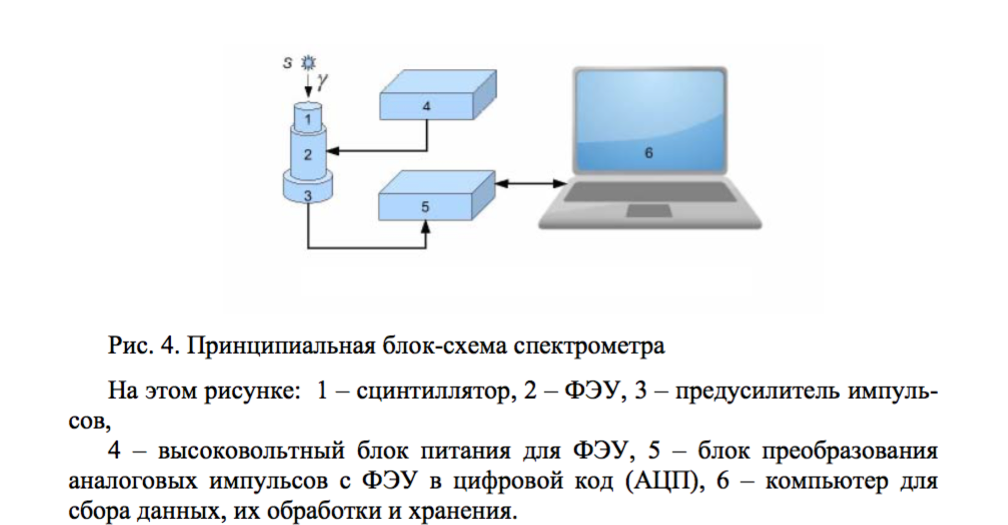
\includegraphics[width=\linewidth]{555computer}
	\end{figure}
	
	
	\section{Ход работы}
	\begin{enumerate}
		\item Подготовили приборы к измерениям
		
		\item Провели измерения для Cs, Co, Eu, Na, Am. Для каждого материала находили положение фотопика. Сначала мы определяли положение пиков приближенно, подводя репер к максимуму и снимая с него координату. Затем, каждый пик аппроксимировали гауссианом и уже из математической функции определяли положение максимума, а также ширину фотопика. Результаты измерений занесли в таблицу:
		
		    \begin{table}[h!]
		    	\centering
		    	\label{my-label}
		    	\begin{tabular}{|l|l|l|l|l|l|l|}
		    		\hline
		    		Элемент & I пик, кан &II пик, кан &IГ пик, кан &$\Delta$I, кан &IIГпик, кан&$\Delta$II, кан \\ \hline
		    		Eu-152 &128,7 &224,1&129,55&43,2&224,21&39,6\\ \hline
		    		Am-241 &112,8&154,8&113,17&27,9&153,09&43,7\\ \hline
		    		Cs-137 &843,1&--&844,095&124,8&--&--\\ \hline
		    		Na-22 &670,5&1516,3&670,43&122,9&1512,3&139\\ \hline
		    		Co-60 &1422,1&1586,2&1417,51&119,6&1586,30&152,7\\ \hline
		    	\end{tabular}
		    	\caption{Таблица результатов}
		    \end{table}
		    
		\item Построим калибровочный график на основе полученных данных
			 \begin{figure}
			 	\centering
			 	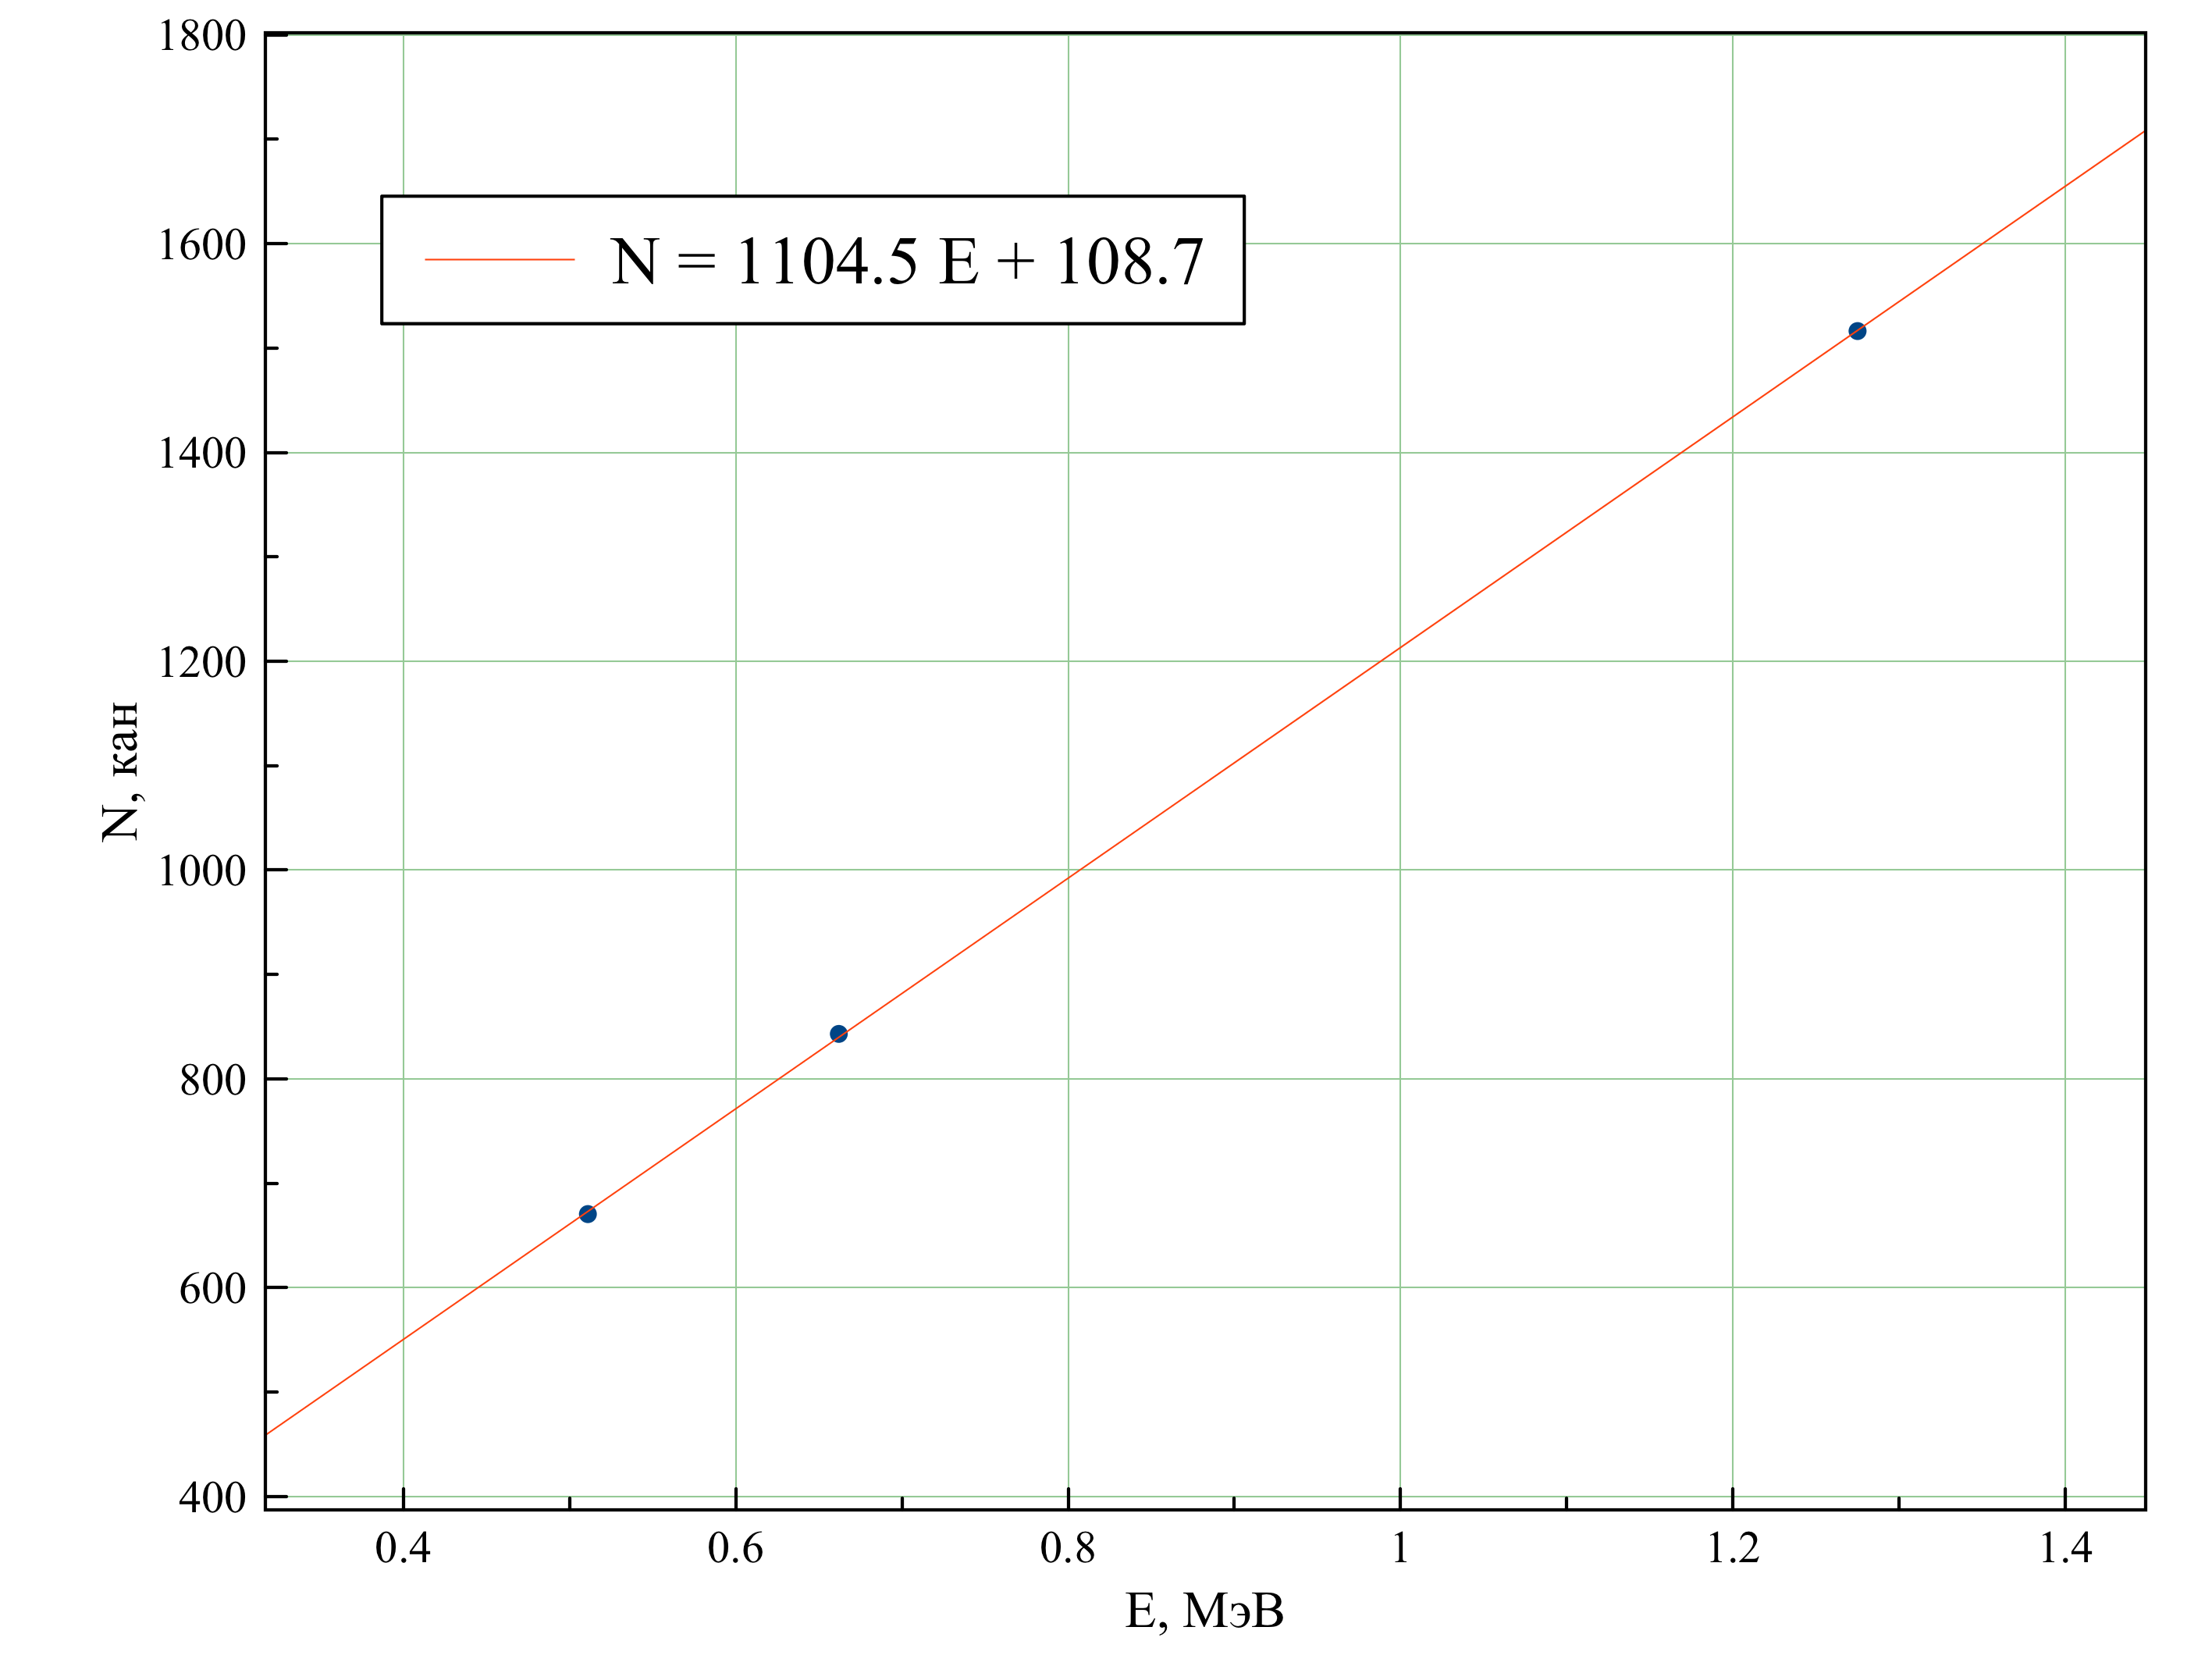
\includegraphics[width=0.8\linewidth]{calib}
			 		\caption{Калибровочный график}
			 \end{figure}
			
			
			\item Приведем результаты пересчета энергии из единиц "каналов" в МэВ
			
			\begin{table}[h!]
				\centering
				\label{my-label}
				\begin{tabular}{|l|l|l|l|l|l|l|l|l|}
					\hline
					Элемент & I пик, кан &$\Delta$I, кан  &E, МэВ &$\Delta$E, МэВ &R&$E_{exp}$, МэВ &$E_{theor}$, МэВ&$E_{inv}$, МэВ\\ \hline
					Eu-152 &129,55&43,2&0,0189&--&--&--&--&0.0176\\ \hline
					Am-241 &113,17&27,9&0,004&--&--&--&--&0.0039\\ \hline
					Cs-137 &844,095&124,8&0,666&0,0146&0.022&0,444&0,483&0.185\\ \hline
					Na-22 &670,43&122,9&0,509&0,0129&0.025&0,309&0,341&0.170\\ \hline
					Co-60 &1417,51&119,6&1,185&0,0099&0.0083&1,0&0,978&0.210\\ \hline
				\end{tabular}
				\caption{Таблица результатов в пересчете}
			\end{table}
			
			
			
			\item  Построим график зависимости теоретического значения комптоновского края от экспериментального: 
		
			
			\begin{figure}
				\centering
				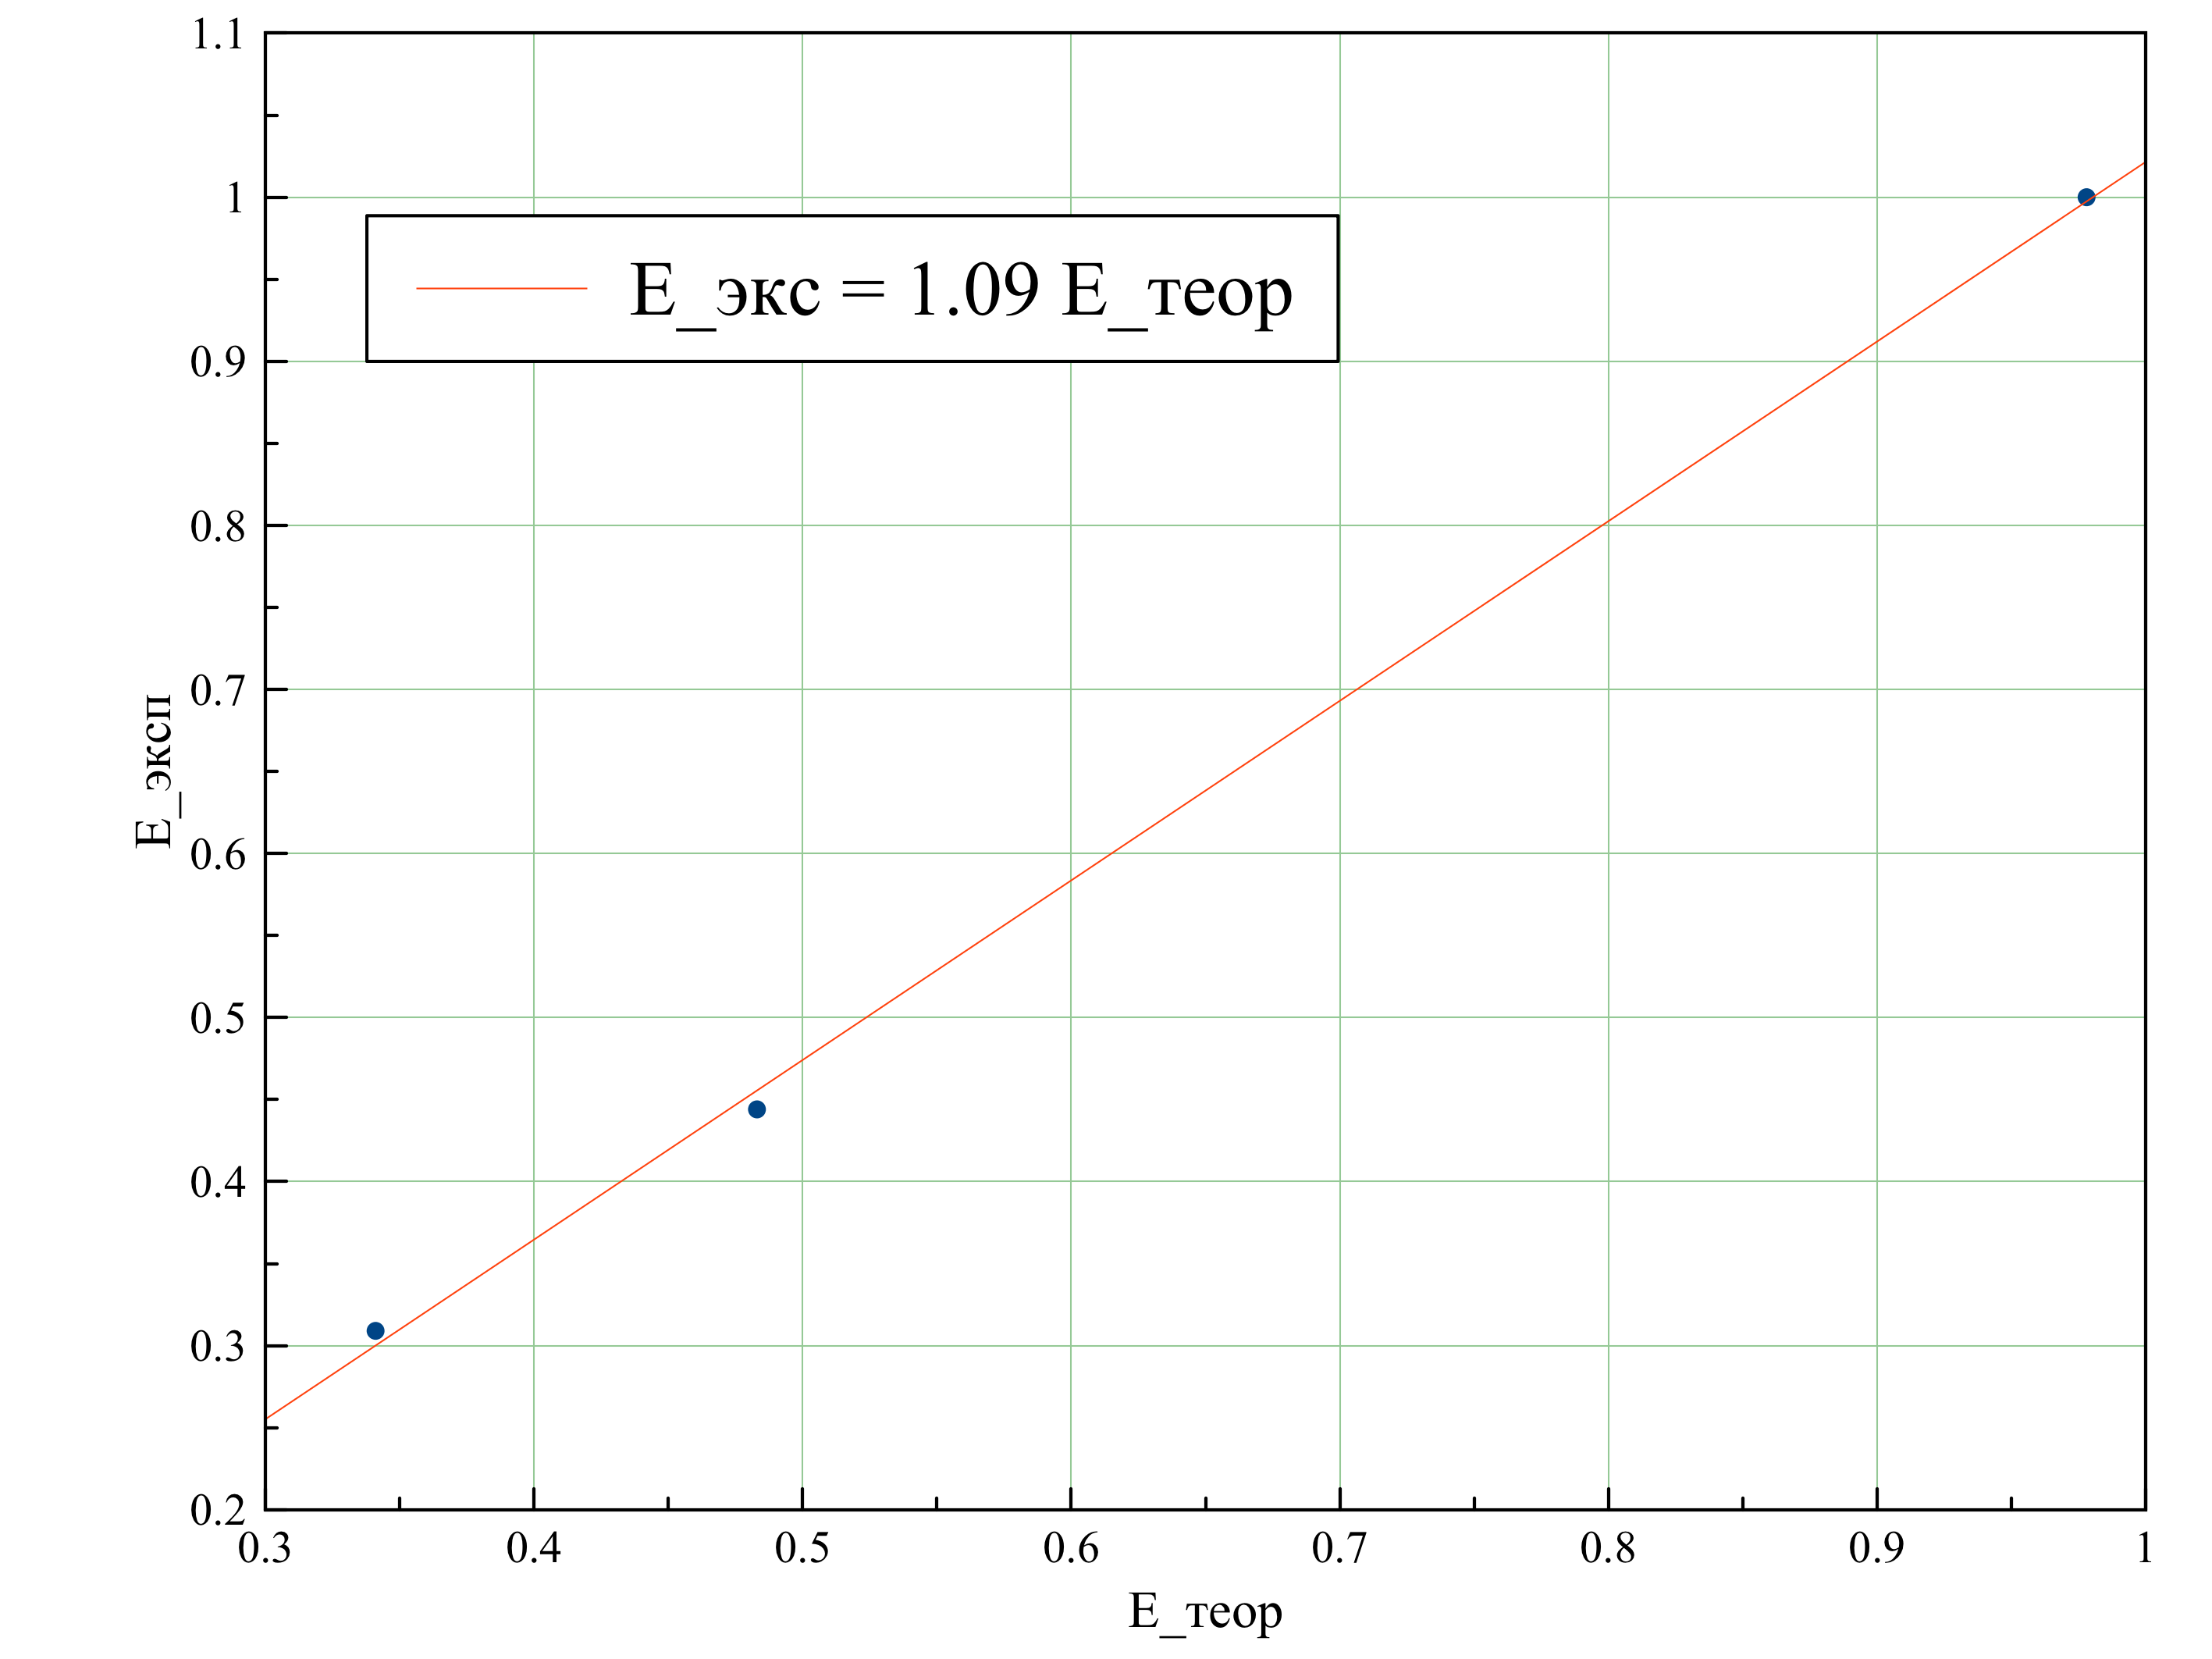
\includegraphics[width=0.7\linewidth]{kompt}
				\caption{Комптоновские края}
			\end{figure}
			
			\item 	 Построим график зависимости энергетического разрешения спектрометра от обратной энергии.
				
			\begin{figure}
				\centering
				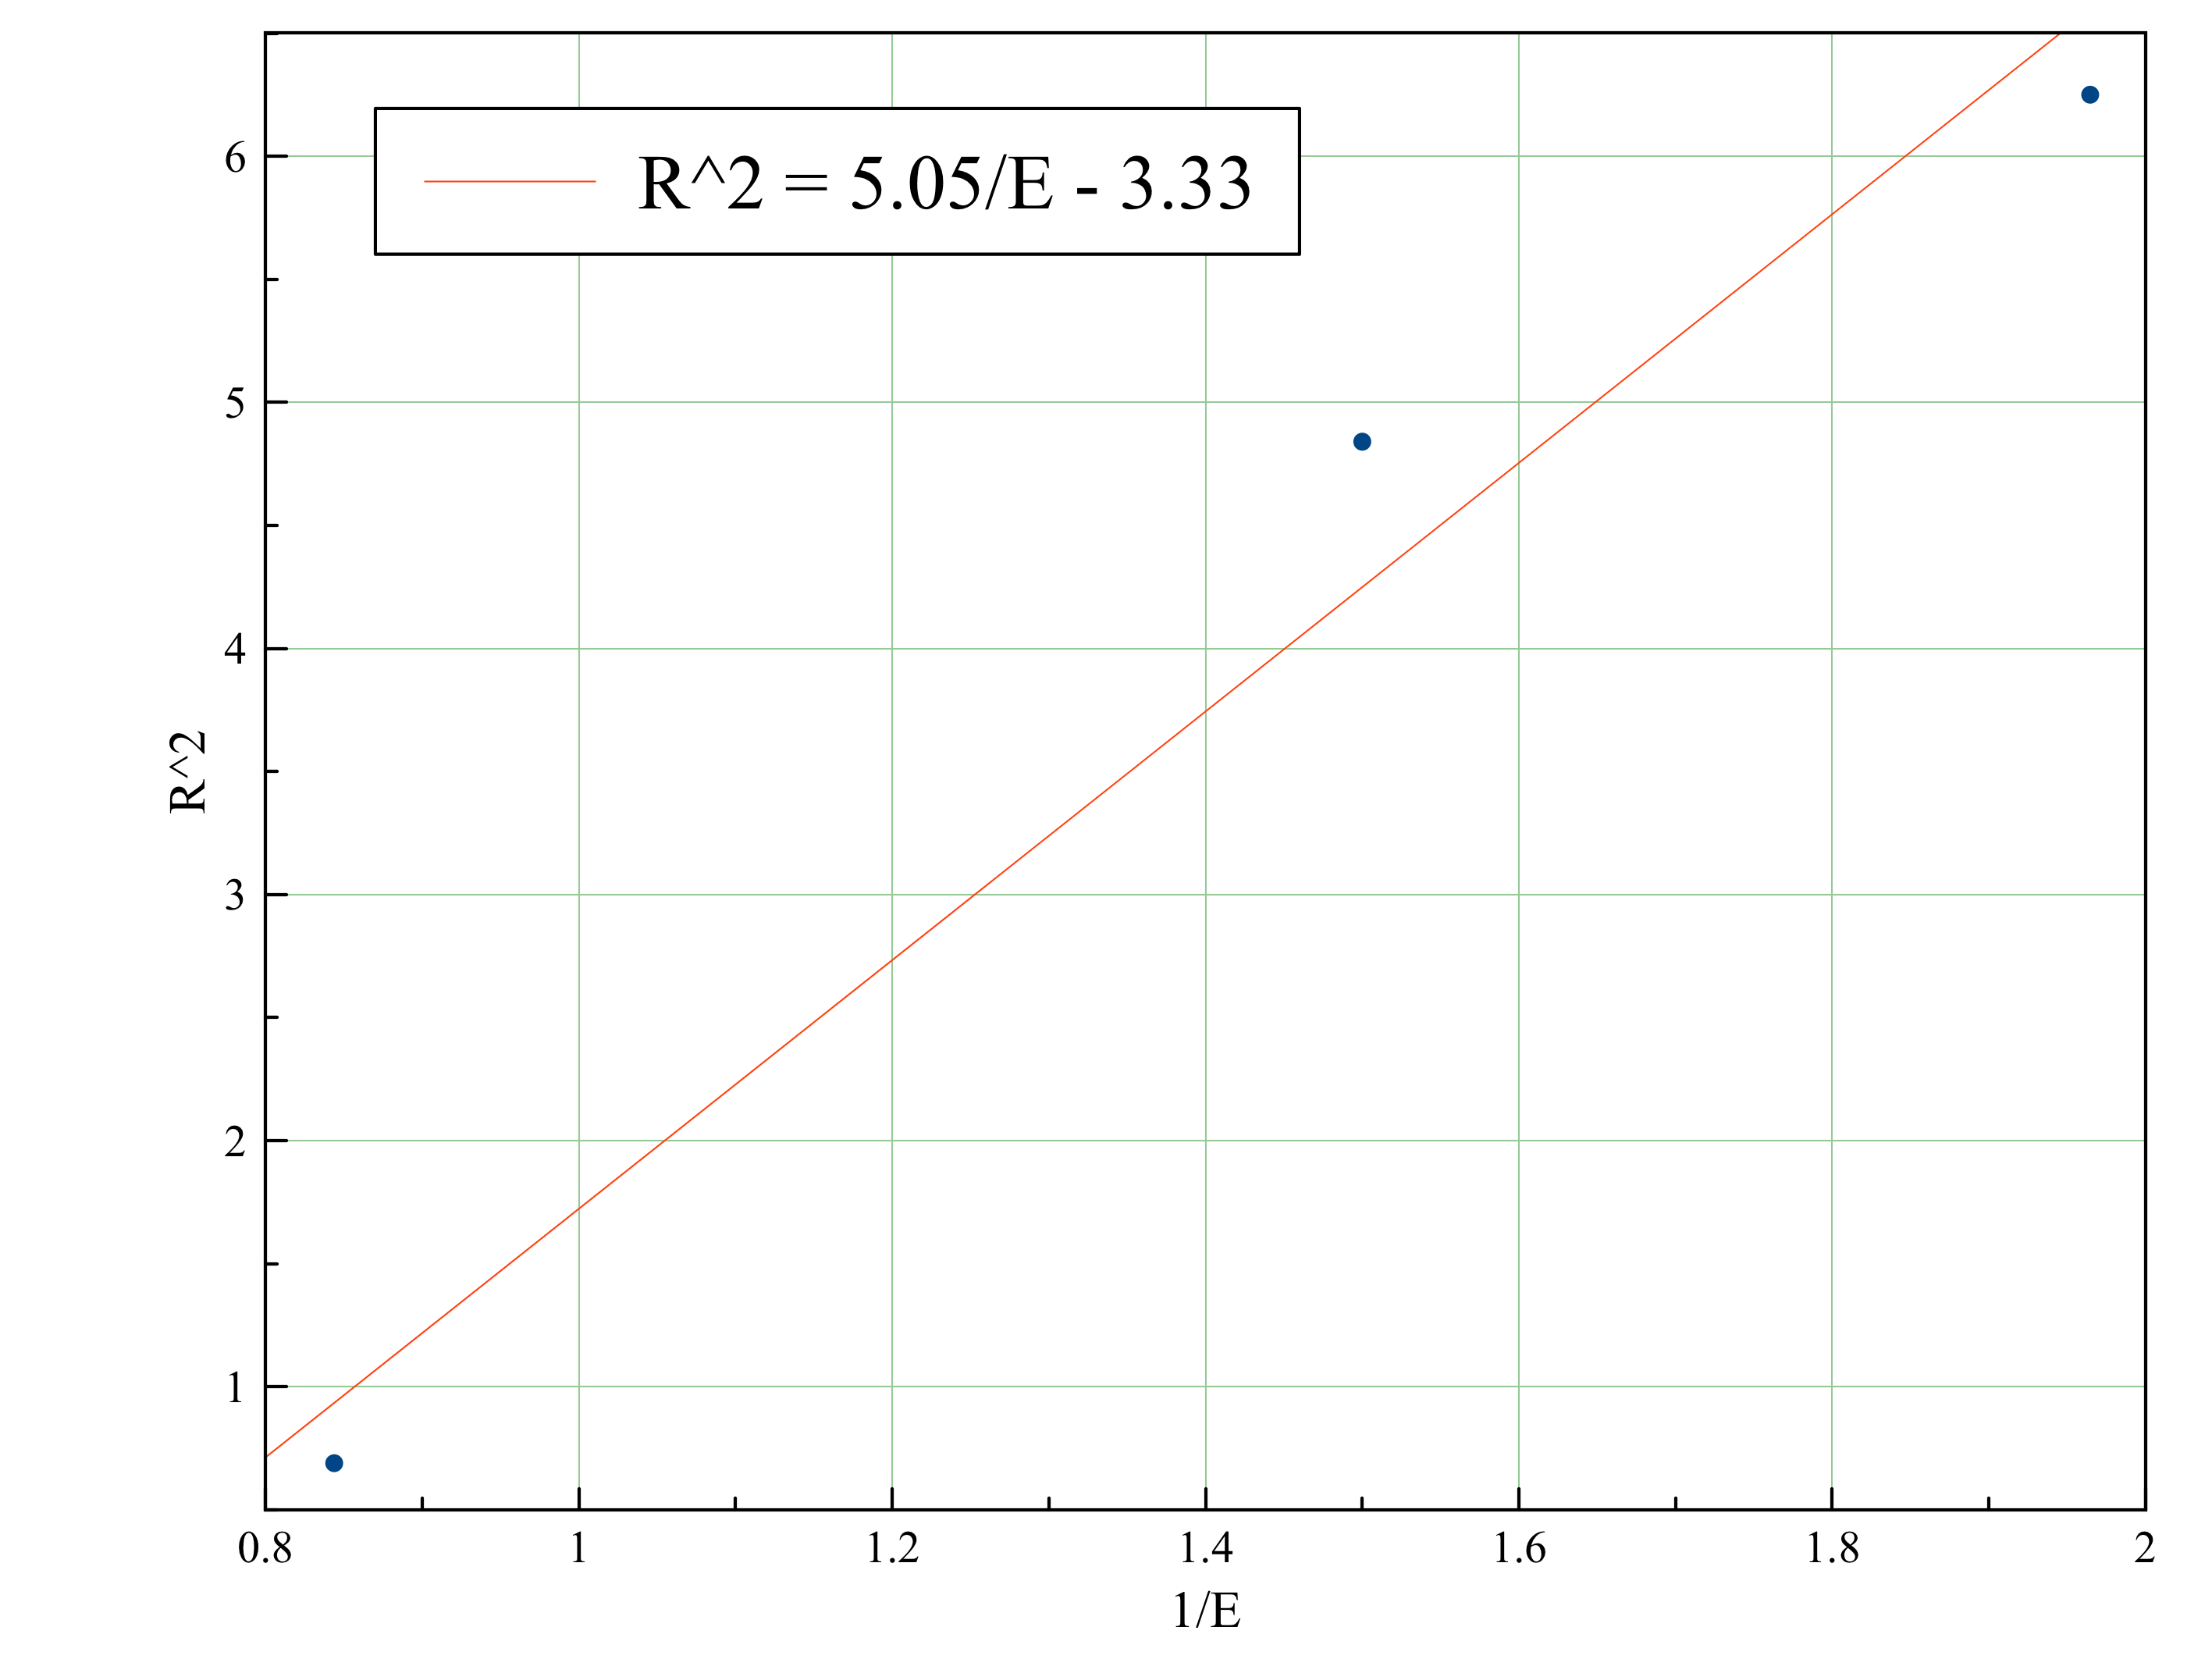
\includegraphics[width=0.8\linewidth]{res}
				\caption{Разрешение}
			\end{figure}
			
			
					\item  Построим график зависимости энергии обратного пика рассеяния от энергии:
					
					\begin{figure}
						\centering
						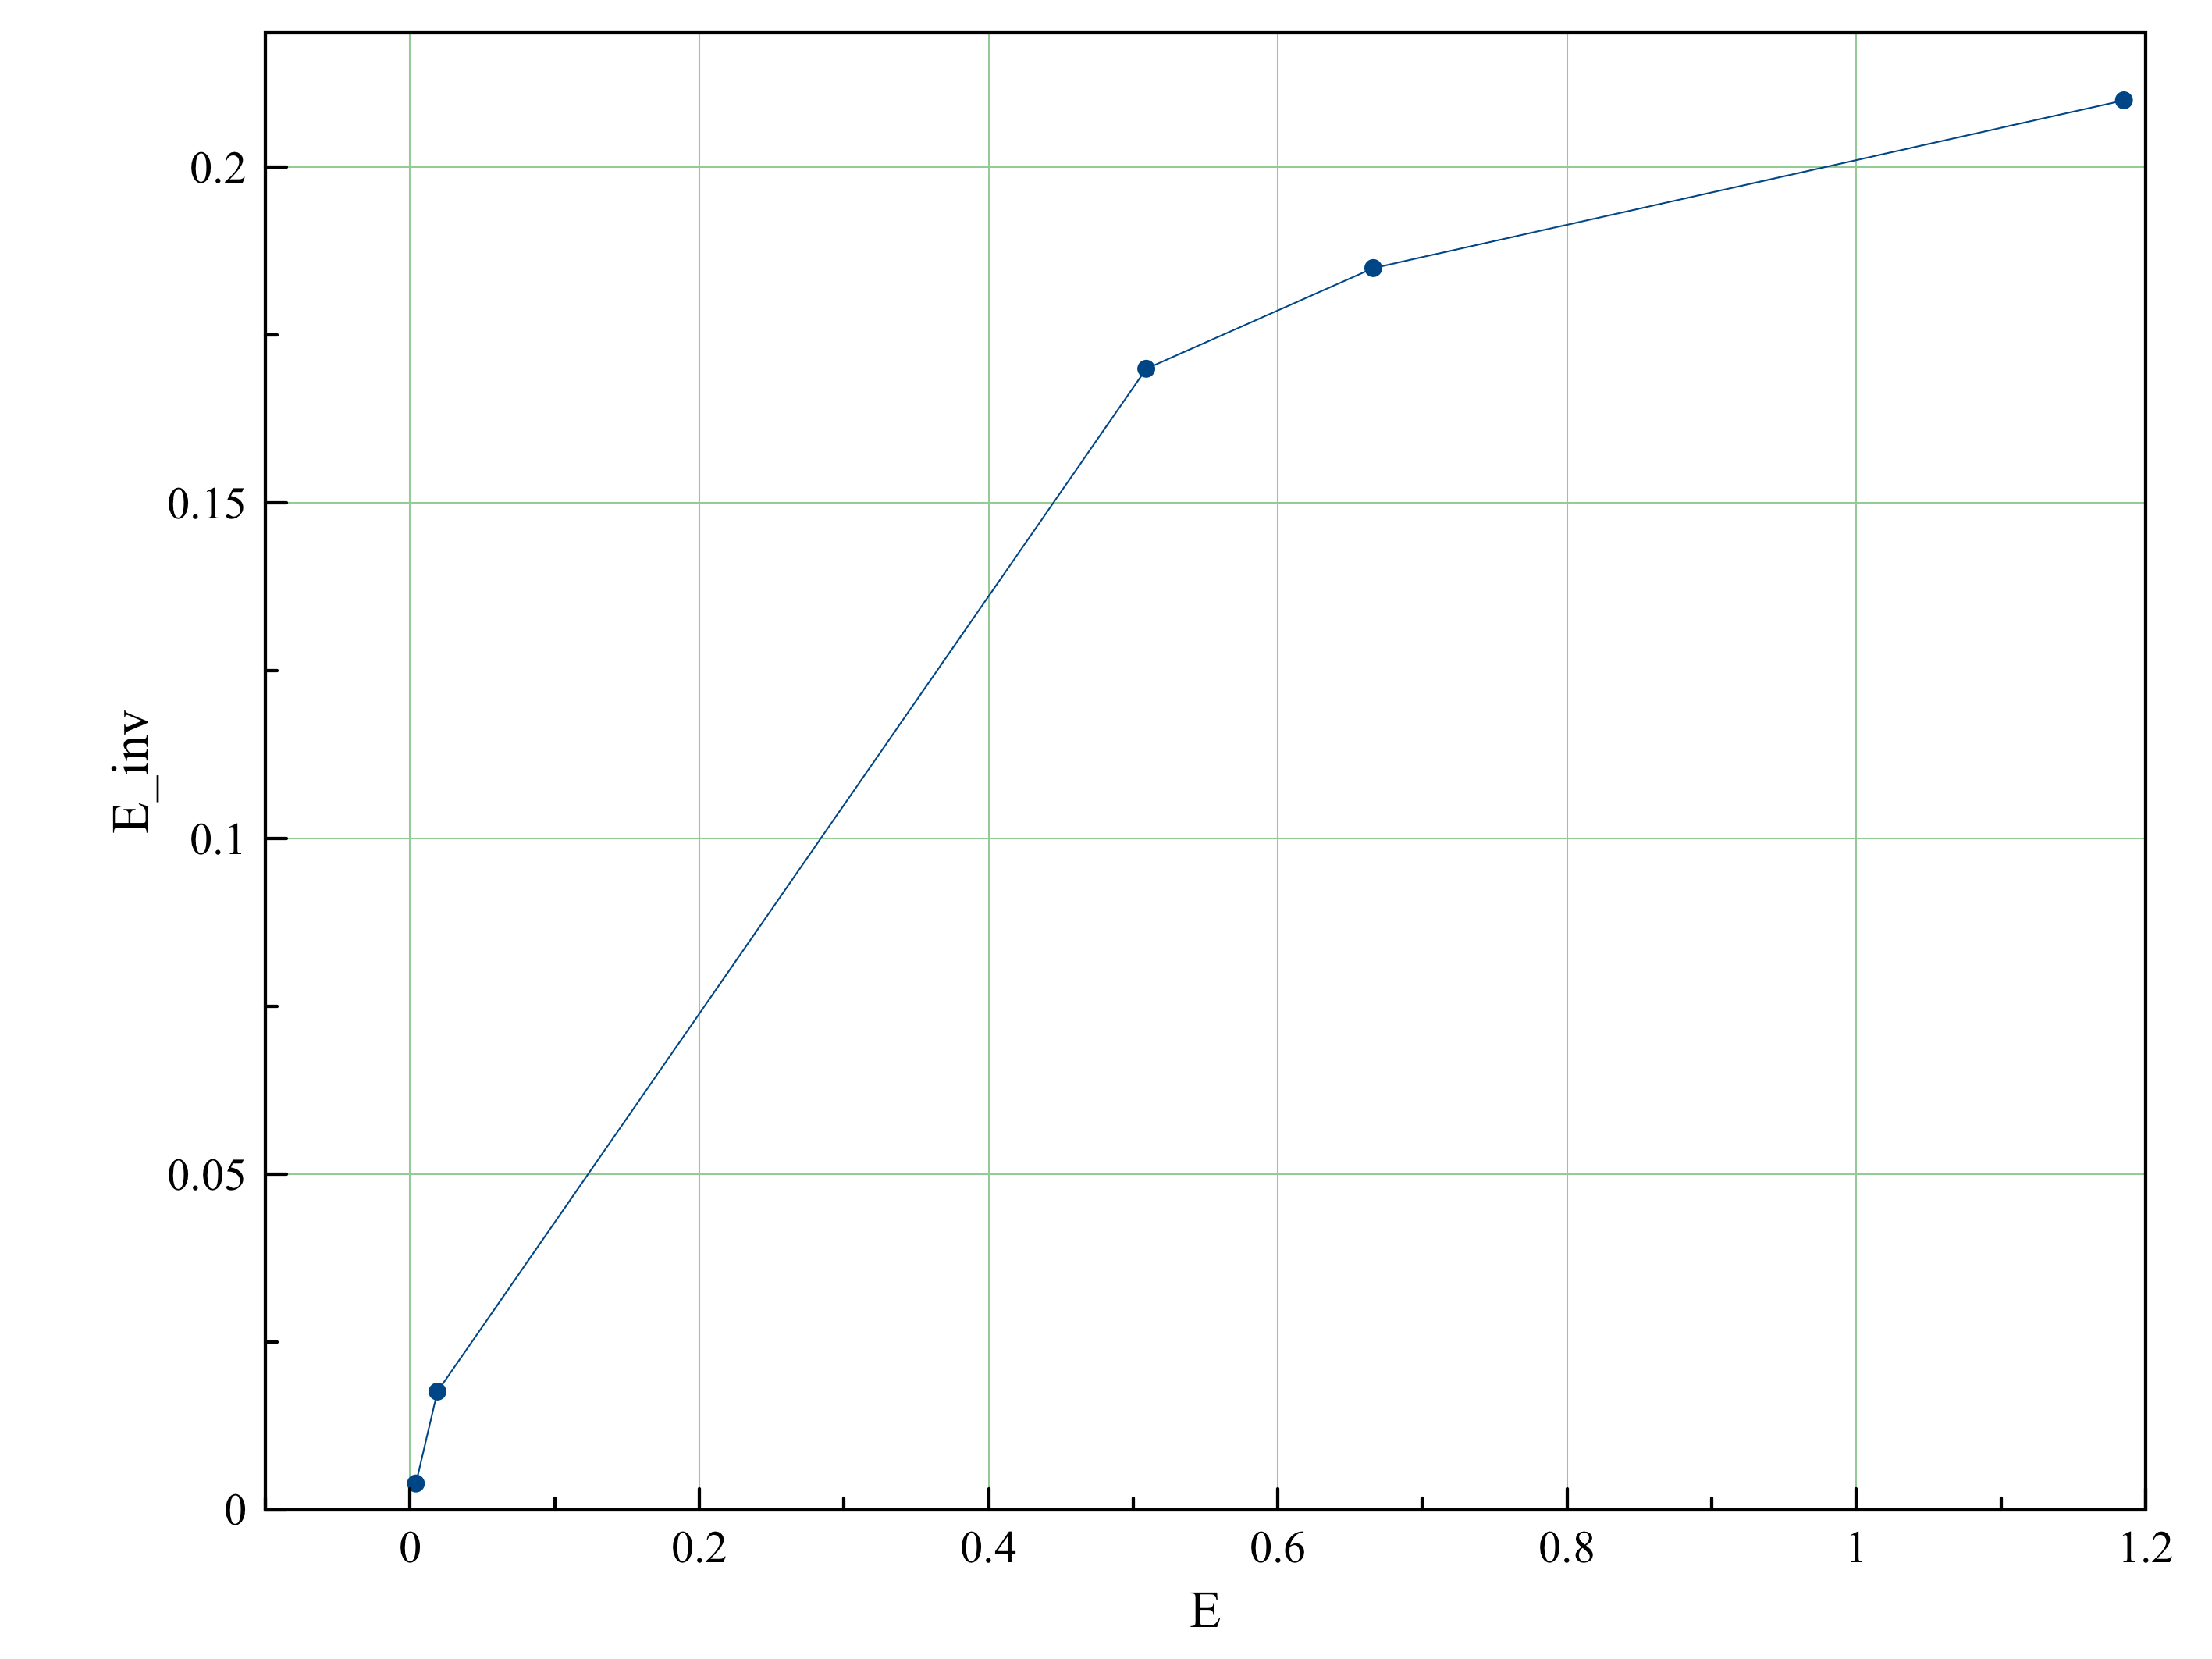
\includegraphics[width=0.7\linewidth]{E_inv}
						\caption{Энергии обратного пика рассеяния от энергии}
						\label{fig:my_label}
					\end{figure}
	\end{enumerate}

	
	
	
	\section{Вывод}
		В данной работе мы исследовали гамма-линии спектров для 5 различных образцов с помощью сцинтиллятора, энергию края комптоновского поглощения  -- теоретические выкладки очень хорошо легли на экспериментальные расчеты.
	
	\newpage
	 \begin{figure}[h!]
	 	\centering
	 	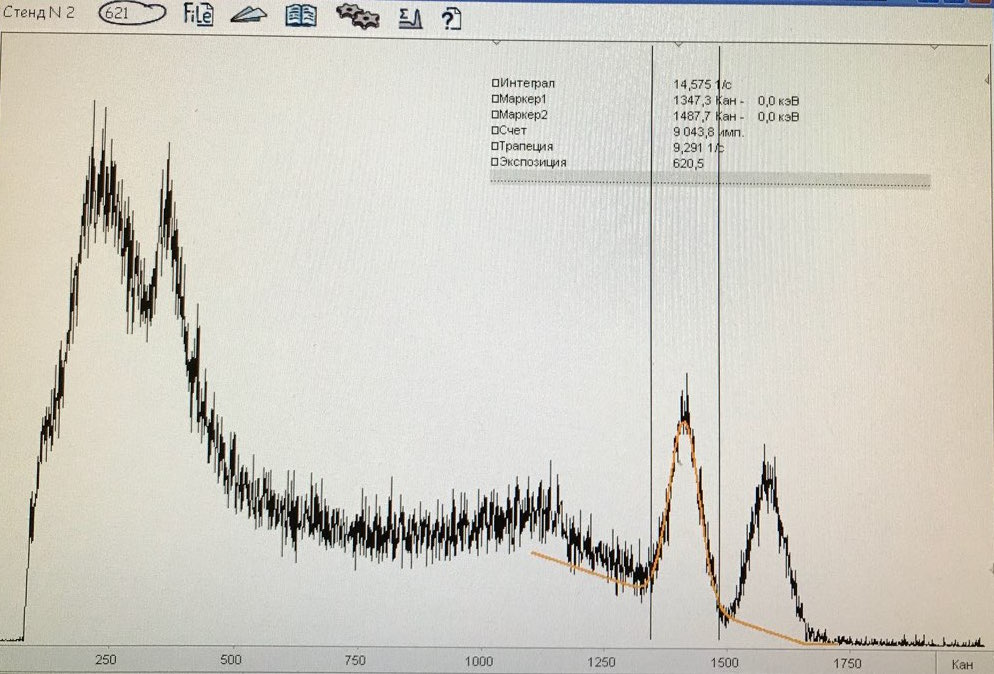
\includegraphics[width=0.9\textwidth]{Co.jpg}
	 	\caption{Спектр $^{60}Co$}
	 \end{figure}
	 
	 \begin{figure}[h!]
	 	\centering
	 	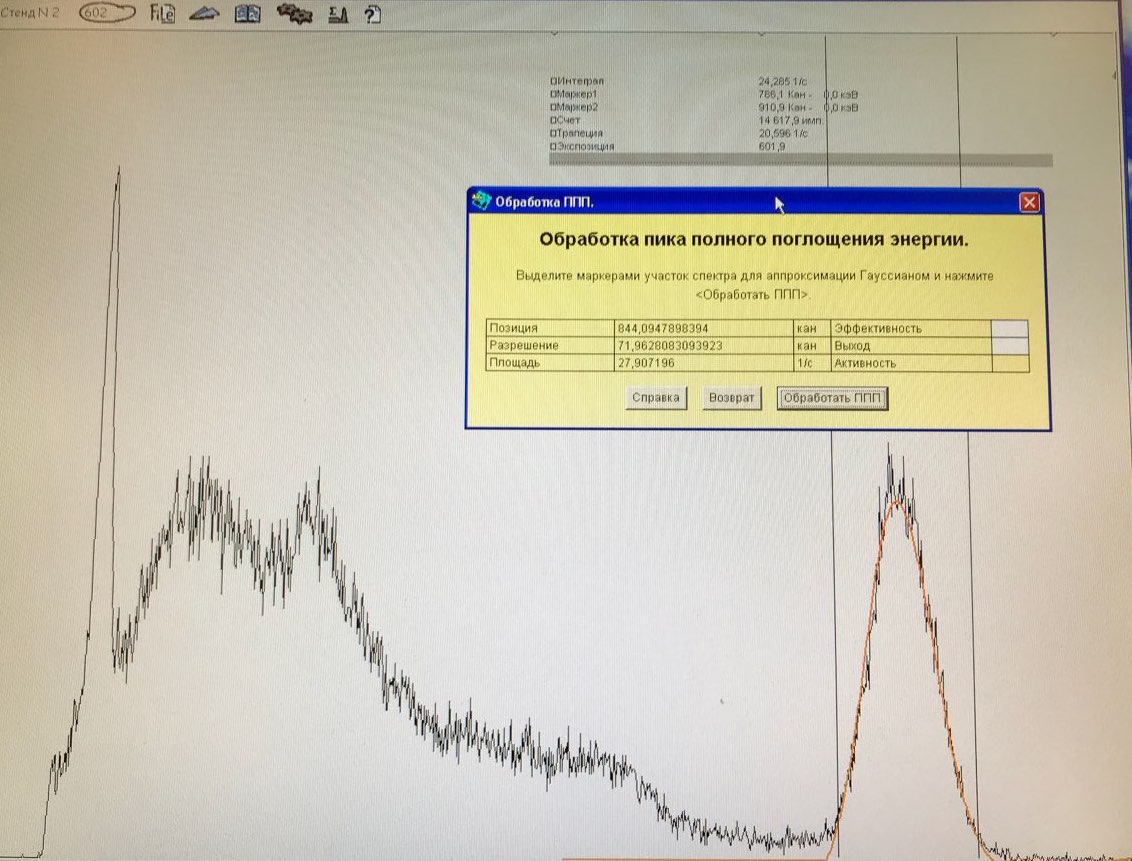
\includegraphics[width=0.9\textwidth]{Cs.jpg}
	 	\caption{Спектр $^{137}Cs$}
	 \end{figure}
	 
	 	 \begin{figure}[h!]
	 	 	\centering
	 	 	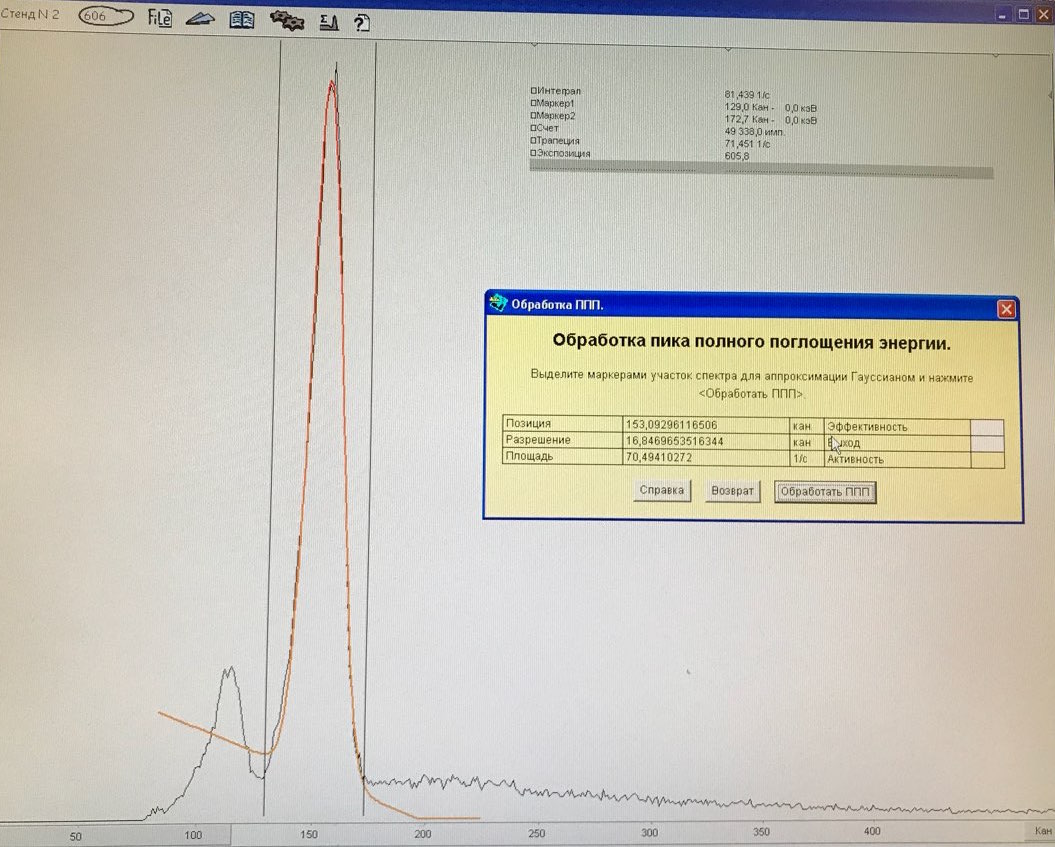
\includegraphics[width=0.9\textwidth]{Am.jpg}
	 	 	\caption{Спектр $^{241}Am$}
	 	 \end{figure}
	 	 
	 \begin{figure}[h!]
	 	\centering
	 	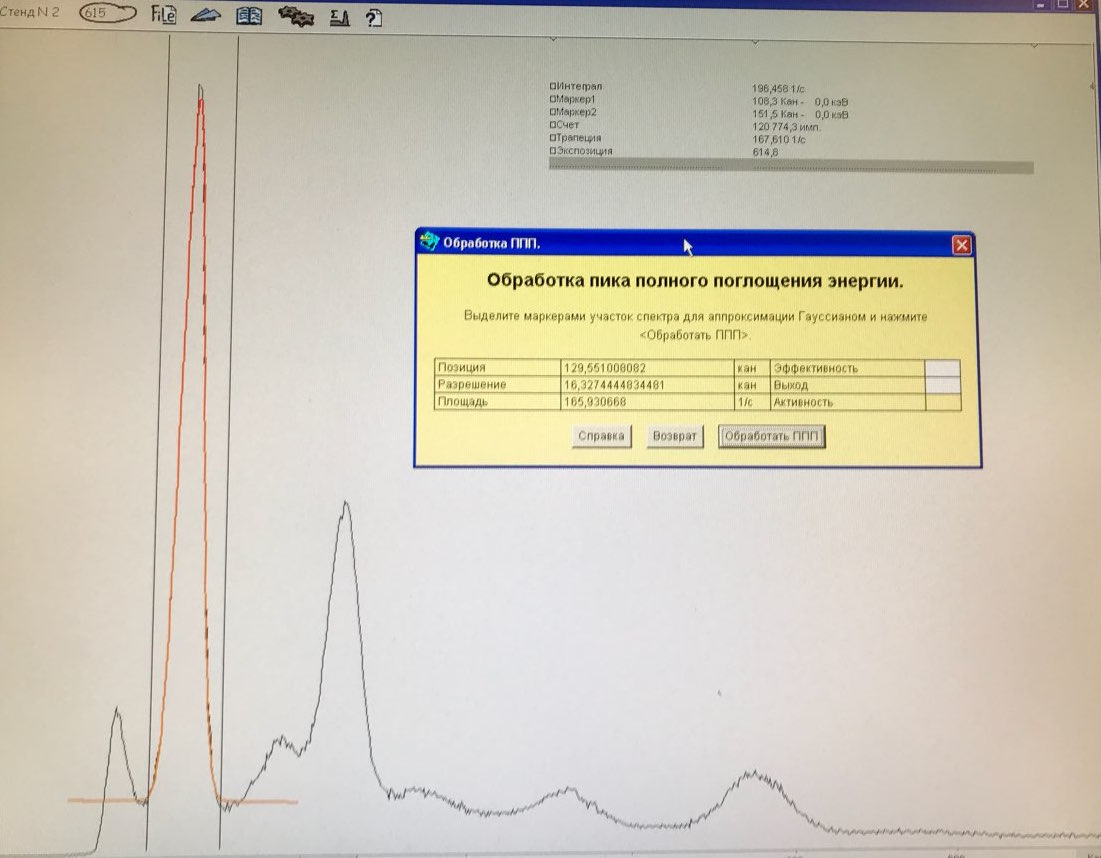
\includegraphics[width=0.8\textwidth]{Eu.jpg}
	 	\caption{Спектр $^{152}Eu$}
	 \end{figure}
	 
	 \begin{figure}[h!]
	 	\centering
	 	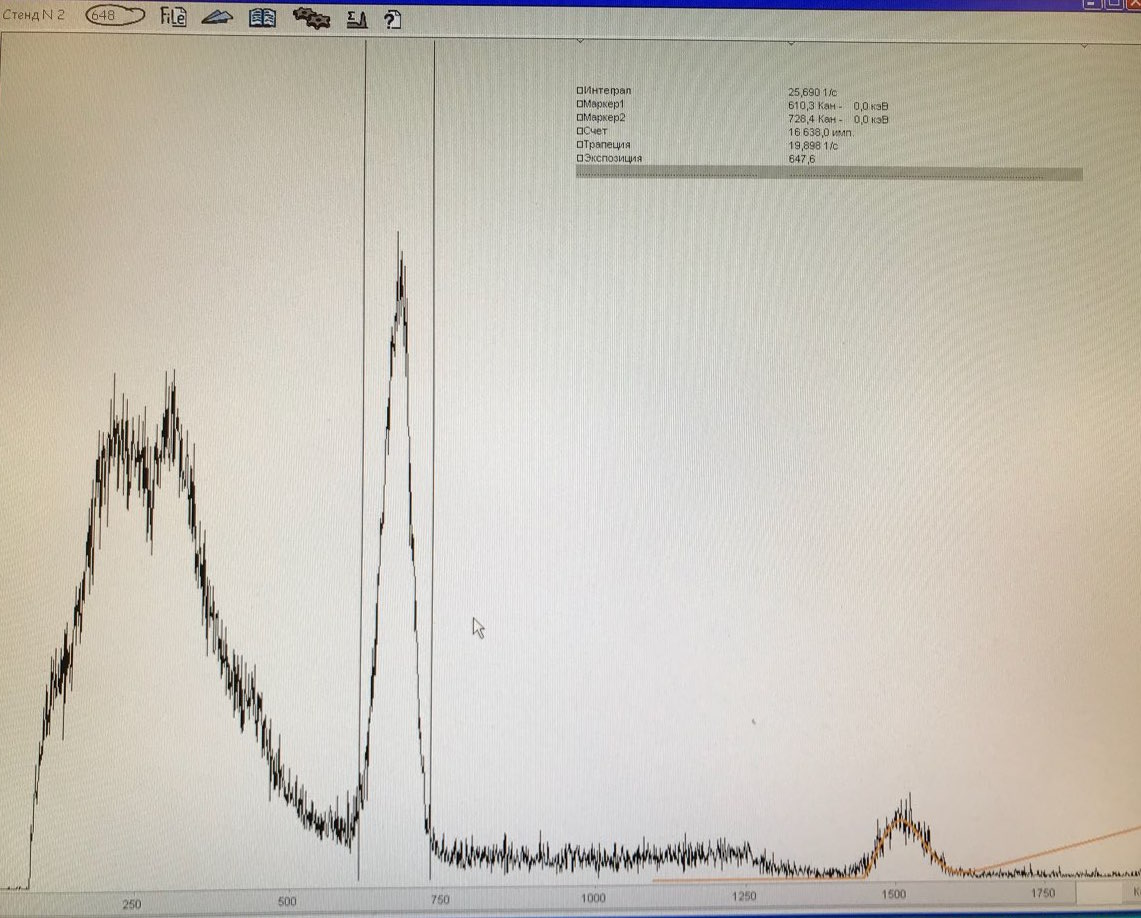
\includegraphics[width=0.9\textwidth]{Na.jpg}
	 	\caption{Спектр $^{22}Na$}
	 \end{figure}
	 
	 
\end{document}


